% College Lecture 17: entity authentication (34 slides) + Forouzan ch. 14 + Stallings (user authentication, UNIX salt).
% Every number recomputed by script (scratchpad/w22/verify*.py): dictionary costs, Lamport chain, FS/FFS/GQ rounds, FAR/FRR.
\section{Entity Authentication}\label{sec:entityauth}
\tikzset{
  eaparty/.style={draw, fill=acc!10, rounded corners=2pt, font=\small\bfseries, align=center, inner sep=3pt, minimum width=2.3cm},
  eamsg/.style={-{Stealth[length=2mm]}, thick},
  eanum/.style={circle, fill=black!85, text=white, font=\scriptsize\bfseries, inner sep=0pt, minimum size=3.8mm},
  eacomp/.style={draw, fill=gray!10, font=\footnotesize, align=left, inner sep=2.5pt, rounded corners=1pt},
  ealab/.style={font=\footnotesize, fill=white, inner sep=1.5pt, above=0pt}
}
% \eaHeads{left}{right}{width}{bottom y}; \eaR / \eaL{y}{number}{label}{width}: message left->right / right->left
\providecommand{\eaHeads}[4]{\node[eaparty] at (0,0.6) {#1}; \node[eaparty] at (#3,0.6) {#2};
  \draw[gray!70, thick] (0,0.12) -- (0,#4); \draw[gray!70, thick] (#3,0.12) -- (#3,#4);}
\providecommand{\eaR}[4]{\draw[eamsg] (0,#1) -- node[ealab]{#3} (#4,#1); \node[eanum] at (0,#1) {#2};}
\providecommand{\eaL}[4]{\draw[eamsg] (#4,#1) -- node[ealab]{#3} (0,#1); \node[eanum] at (#4,#1) {#2};}
\providecommand{\eaA}{Alice\\[-2pt]{\footnotesize\mdseries (claimant)}}
\providecommand{\eaB}{Bob\\[-2pt]{\footnotesize\mdseries (verifier)}}

\subsection{What entity authentication is \new}
\likely{``Define entity authentication; differentiate data-origin (message) authentication and entity authentication'' (2--3 marks).}

\textbf{Entity authentication} is a technique designed to let one party prove the identity of another party. An \textbf{entity} can be a person, a process, a client or a server. \imp{The entity whose identity needs to be proved is called the claimant; the party that tries to prove the identity of the claimant is called the verifier.} When Bob tries to prove the identity of Alice, Alice is the claimant and Bob is the verifier. The proof always rests on a \textbf{witness}: something that only the true Alice can show or compute, and that Bob can check.

\textbf{Data-origin versus entity authentication.} Message authentication (data-origin authentication, provided by a MAC or a digital signature) also tells Bob who created something, so the two ideas are easily confused. The slides give two differences.
\begin{itemize}
  \item \textbf{Real time.} Message authentication might not happen in real time; entity authentication does. When Bob authenticates an e-mail from Alice, she may or may not be present; the MAC or signature travelled with the message and can be checked days later. When Alice requests entity authentication, no real message is communicated until Bob has authenticated her: she must be online and take part in the process, and only afterwards can messages flow. Data-origin authentication is needed when an e-mail is sent; entity authentication is needed when Alice draws cash from an ATM.
  \item \textbf{One message versus a session.} Message authentication authenticates one message, so the process must be repeated for each new message. Entity authentication authenticates the claimant for the entire duration of a session.
\end{itemize}
A consequence of the first difference is that entity authentication must defeat \textbf{replay}. A signed e-mail replayed a week later is still a genuine message from Alice, so its signature still checks; but a recorded login replayed a week later must \emph{not} make Bob believe Alice is present now. Every protocol in this section therefore contains something that changes from one run to the next (a one-time password, a nonce, a timestamp, a fresh random commitment).
\begin{center}\small
\begin{tabularx}{\textwidth}{@{}l X X@{}}
\toprule
 & Data-origin (message) authentication & Entity authentication\\
\midrule
Question answered & Who created \emph{this message}? & Who is at the other end \emph{now}?\\
Real time & Not necessarily; the sender may be offline & Yes; the claimant takes part online\\
Scope & One message; repeated for every message & Whole session, done once at the start\\
Replay & A replayed message is still authentic & A replayed proof must be rejected (freshness)\\
Mechanisms & MAC, HMAC, digital signature & Passwords, challenge--response, zero-knowledge, biometrics\\
Example & Alice e-mails Bob & Alice withdraws cash at an ATM; login\\
\bottomrule
\end{tabularx}
\end{center}

\subsection{Verification categories and multi-factor authentication \new}
\likely{``What are the three kinds of witness? Give examples'' (2 marks); ``why is ATM card + PIN stronger than either alone?''}

The claimant must identify herself to the verifier with one of three kinds of witnesses.
\begin{itemize}
  \item \textbf{Something known}: a secret known only by the claimant that the verifier can check. Examples are a password, a PIN, a secret key and a private key.
  \item \textbf{Something possessed}: an object that proves the claimant's identity. Examples are a passport, a driver's licence, an identification card, a credit card and a smart card.
  \item \textbf{Something inherent}: an inherent characteristic of the claimant. Examples are a conventional signature, fingerprints, voice, facial characteristics, the retinal pattern and handwriting.
\end{itemize}
Stallings splits the third category in two, giving four means: something the individual \emph{knows}, \emph{possesses}, \emph{is} (static biometrics: fingerprint, retina, face) and \emph{does} (dynamic biometrics: voice pattern, handwriting, typing rhythm). The two classifications agree; Stallings only separates physiological from behavioural features.

\textbf{Multi-factor authentication.} Each category fails in its own way: a known secret can be guessed or observed, a possessed object can be stolen or lost, an inherent feature can be copied and never changed. Combining witnesses from \emph{different} categories forces Eve to mount two unrelated attacks at once; stealing the card does not reveal the PIN, and watching the PIN being typed does not produce the card. \imp{Two-factor authentication means two witnesses from two different categories}; two passwords are still one factor, because one keylogger captures both. Everyday examples are an ATM card with a PIN (possessed + known), a password with a one-time code sent to the registered phone (known + possessed), UPI, where the phone with its bound SIM is possessed and the UPI PIN is known, and Aadhaar authentication with a fingerprint plus an OTP (inherent + possessed).

\subsection{Fixed passwords: the four approaches \new}
\likely{``Explain hashing and salting of passwords; what is a dictionary attack and how does salting make it harder?'' (4--5 marks), often with the slide figure.}

The simplest and oldest method of entity authentication is \textbf{password-based authentication}, where the password is something that the claimant knows. A password is used when a user needs to access a system to use its resources (login). Each user has a \textbf{user identification} (user ID) that is public and a \textbf{password} that is private. Password schemes fall into two groups: the \textbf{fixed password}, which is used over and over again for every access, and the \textbf{one-time password}, which is used only once. Several fixed-password schemes have been built, each one repairing a weakness of the previous one.

\begin{center}
\begin{tikzpicture}[font=\small]
\eaHeads{\eaA}{\eaB}{5.5}{-1.5}
\eaR{-0.7}{1}{Alice, \textit{Pass}}{5.5}
\node[eacomp, anchor=west] at (5.85,-0.7) {\begin{tabular}{@{}lll@{}}
  \multicolumn{3}{@{}l}{look up Alice's row of the password file; grant access iff}\\
  1st approach: & \textit{Pass} $= P_A$ & file row: Alice, $P_A$\\
  2nd approach: & $h(\mathit{Pass}) = h(P_A)$ & file row: Alice, $h(P_A)$\\
  3rd approach: & $h(\mathit{Pass}\,\|\,S_A) = h(P_A\,\|\,S_A)$ & file row: Alice, $S_A$, $h(P_A\,\|\,S_A)$\end{tabular}};
\end{tikzpicture}
\end{center}
$P_A$ is Alice's stored password, \textit{Pass} the password sent by the claimant, $S_A$ Alice's salt and $\|$ concatenation. The message is the same in all three approaches; they differ only in what the verifier stores and computes.

\textbf{First approach: user ID and password file.} The system keeps a table (file) sorted by user ID, with the password of each user stored in clear. To access the system, Alice sends her user ID and password; the system uses the ID to find her row and compares the stored password $P_A$ with the received \textit{Pass}. If they match, access is granted; otherwise it is denied. The approach is open to four attacks.
\begin{itemize}
  \item \textbf{Eavesdropping}: Eve watches Alice while she types her password (or listens on the line). As a measure, most systems do not echo the characters typed.
  \item \textbf{Stealing a password}: Eve physically steals the password, for example a note on which Alice wrote it. This is prevented if Alice does not write the password down but commits it to memory.
  \item \textbf{Accessing the password file}: Eve hacks into the system and reads the ID/password file, which gives her every user's password at once. The file can be read/write protected, but one bug or one dishonest administrator defeats the protection.
  \item \textbf{Guessing}: Eve logs into the system and tries different combinations of characters as Alice's password. This works well if Alice chose something trivial such as her birthday, her child's name or the name of her favourite actor. A long random password is recommended. Online guessing can also be throttled by locking the account or adding a delay after a few failures.
\end{itemize}

\textbf{Second approach: hashing the password.} The third attack is the most damaging because one break exposes every user, so the system stops storing passwords and stores their hashes. When the password is created, the system stores $h(P_A)$ instead of $P_A$; at login it computes $h(\mathit{Pass})$ and compares it with the stored value. Since $h$ is a one-way (preimage-resistant) hash function, Eve cannot recover $P_A$ from $h(P_A)$ even if she reads the whole file, and she cannot log in with $h(P_A)$ itself, because the system will hash whatever she sends.

\textbf{The dictionary attack.} Hashing protects strong passwords but not the ones people actually choose, because the set of likely passwords is small. In a \textbf{dictionary attack}, Eve is interested in finding \emph{one} password, regardless of the user ID. If passwords are 6 digits, she lists all numbers from 000000 to 999999 and hashes every one, which gives a list of one million (word, hash) pairs. She then obtains the password file and searches its second column for any hash in her list; a match gives her the password of that user. All of this can be programmed and run \textbf{offline} on Eve's own computer, so account lock-outs and delays do not slow it down; only after a match does she go online and log in. The cost is one hash per candidate password, and since the same list serves every user and every system that uses the same $h$, it can be computed once and reused.

\begin{worked}[: cost of a dictionary attack]
\textbf{Q.} Eve has stolen a file of unsalted password hashes and can compute $10^9$ hashes per second. How long does an exhaustive dictionary attack take if passwords are (a) 6 decimal digits, (b) 8 lowercase letters, (c) 8 characters from the 95 printable ASCII characters?

\textbf{A.} The work is (number of candidates) $\div$ (rate), and one pass covers all users.\\
(a) $10^6$ candidates: $10^6 / 10^9 = \mathbf{0.001}$ \textbf{s}.\\
(b) $26^8 = 208\,827\,064\,576 \approx 2.09 \times 10^{11}$: $\approx 209$ s $\approx \mathbf{3.5}$ \textbf{minutes}.\\
(c) $95^8 = 6\,634\,204\,312\,890\,625 \approx 6.63 \times 10^{15}$: $6.63 \times 10^{6}$ s $\div 86\,400 \approx \mathbf{77}$ \textbf{days}.\\
\emph{Check}: each extra character multiplies the work by the alphabet size; going from 26 to 95 symbols multiplies it by $(95/26)^8 \approx 3.2 \times 10^4$, which matches $6.63 \times 10^{15} / 2.09 \times 10^{11}$.
\end{worked}

\textbf{Third approach: salting the password.} When the password is created, a random string called the \textbf{salt} is concatenated to the password, and the salted password is hashed. The ID, the salt and the hash are stored in the file: (Alice, $S_A$, $h(P_A \| S_A)$). When a user asks for access, the system extracts her salt, concatenates it with the received password, hashes the result, and compares it with the stored hash. The salt is \emph{not} secret; it is stored in clear next to the hash, because the system needs it at every login.

\textbf{Why salting makes the dictionary attack harder.} Without salt, two users with the same password have the same hash, and a single precomputed list $h(w)$ for every dictionary word $w$ attacks every user in every system at once. With salt, the hash of a word depends on the salt, so a precomputed list must contain $h(w \| S)$ for every word \emph{and every possible salt}: a $b$-bit salt multiplies the size of the list by $2^b$. The slide's example: if the password is 6 digits and the salt 4 digits, hashing is done over a 10-digit value, and a complete precomputed list has $10^{10}$ entries instead of $10^6$. Stallings lists three effects of the salt.
\begin{itemize}
  \item It prevents duplicate passwords from being visible in the password file: two users with the same password get different salts and therefore different hashes.
  \item It greatly increases the difficulty of offline dictionary attacks: with a $b$-bit salt, the number of possible hashed values for each password grows by a factor of $2^b$, so precomputed tables become $2^b$ times larger, and the users of one file must be attacked one at a time.
  \item It becomes nearly impossible to find out whether a person with accounts on two or more systems has used the same password on all of them.
\end{itemize}
In \textbf{UNIX} the salt is 12 bits, so each password can be stored in $2^{12} = 4096$ different ways; the classical \texttt{crypt} also iterates its DES-based one-way function 25 times to make each guess slower. \textbf{What salting does not do}: if Eve attacks one particular user, she reads that user's salt from the file and hashes her dictionary with it, which costs exactly as much as an unsalted attack. Salting therefore defeats precomputation and attacks on many users at once, but a weak password of a single targeted user still falls; against that, the only defences are long random passwords and a deliberately slow hash (many iterations, as in \texttt{crypt}, PBKDF2 or bcrypt).

\begin{worked}[: what a 12-bit salt buys]
\textbf{Q.} A system with 1000 users stores salted hashes with a 12-bit salt. Eve's dictionary has $10^6$ words and she computes $10^6$ hashes per second. Compare (a) the size of a precomputed table covering all salts with the unsalted table; (b) the time to test the dictionary against all 1000 users with and without salt; (c) the time to attack Alice alone.

\textbf{A.} (a) Unsalted: $10^6$ entries. Salted: $10^6 \times 2^{12} = 10^6 \times 4096 = \mathbf{4.096 \times 10^9}$ entries, 4096 times larger.\\
(b) Unsalted: one pass of $10^6$ hashes; each digest is looked up among the 1000 stored hashes, so $\mathbf{1}$ \textbf{s} for all users. Salted: the users (almost all) have different salts, so each needs its own pass: $1000 \times 10^6 = 10^9$ hashes $= 1000$ s $\approx \mathbf{16.7}$ \textbf{minutes}.\\
(c) Alice's salt is in the file, so one pass of $10^6$ hashes: still $\mathbf{1}$ \textbf{s}.\\
\emph{Check}: salting multiplied the bulk attack by the number of distinct salts (1000) and precomputation by $2^{12}$, but did not change the single-user attack.
\end{worked}

\textbf{Fourth approach: combining two identification techniques.} Two identification techniques are combined, the standard example being an ATM card with a PIN (personal identification number). The card belongs to the category ``something possessed'' and the PIN to ``something known''. The PIN is a password that enhances the security of the card: if the card is stolen, it cannot be used unless the PIN is known. The PIN, however, is traditionally very short (4 digits, $10^4$ values) so that it is easily remembered, which makes it vulnerable to guessing; the card is therefore retained or blocked after three wrong PINs, which turns a $1/10^4$ chance per try into at most a $3/10^4$ chance overall.

\begin{center}\small
\begin{tabularx}{\textwidth}{@{}l l X@{}}
\toprule
Approach & File stores & Remaining weakness\\
\midrule
1. Password file & ID, $P_A$ & Stolen file reveals every password; eavesdropping; guessing\\
2. Hashing & ID, $h(P_A)$ & Offline dictionary attack with one precomputed list for all users\\
3. Salting & ID, $S_A$, $h(P_A \| S_A)$ & Weak password of one targeted user still falls; eavesdropping\\
4. Two techniques & card data, PIN check & Short PIN guessable (hence retry limit); card can be cloned\\
\bottomrule
\end{tabularx}
\end{center}
All four approaches share one weakness: the same password crosses the line at every login, so an eavesdropper who records it once can replay it forever. One-time passwords remove exactly this.

\subsection{One-time passwords and Lamport's hash chain \hot\new}
\likely{``Explain the Lamport one-time password scheme with a diagram; why can an eavesdropper not use what she sees?'' (4--5 marks), possibly with a small hash chain to compute.}

A \textbf{one-time password} is a password that is used only once. Since each value is accepted a single time, recording it is useless: \imp{a one-time password makes eavesdropping and reuse (replay) of the password useless}, and it also makes salting unnecessary, because a stolen value cannot be used again. Forouzan gives three approaches.

\textbf{First approach: an agreed list.} The user and the system agree upon a list of passwords, and each password on the list can be used only once. There are two drawbacks. First, the system and the user must keep a long list of passwords, and whoever steals either copy of the list owns all future logins. Second, if the user does not use the passwords in sequence, the system needs to perform a long search to find the match.

\textbf{Second approach: sequentially updated passwords.} The user and the system agree on an original password $P_1$, which is valid only for the first access. During the first access, the user generates a new password $P_2$ and sends it encrypted with $P_1$ as the key; $P_2$ becomes the password for the second access. During the second access the user generates $P_3$ and encrypts it with $P_2$, and so on: $P_i$ is used to create (carry) $P_{i+1}$.
\begin{center}
\begin{tikzpicture}[font=\small]
\eaHeads{\eaA}{\eaB}{6}{-1.6}
\eaR{-0.8}{$i$}{Alice, $E_{P_i}(P_{i+1})$}{6}
\node[eacomp, anchor=east] at (-0.4,-0.8) {choose a fresh $P_{i+1}$;\\ encrypt it under $P_i$};
\node[eacomp, anchor=west] at (6.4,-0.8) {decrypt with the stored $P_i$; a well-formed\\ result proves Alice knew $P_i$; replace $P_i$ by $P_{i+1}$};
\end{tikzpicture}
\end{center}
The weakness is that the passwords form a chain that can be followed \emph{forwards}. If Eve guesses or steals $P_1$ (or any later $P_i$), she decrypts the recorded message of that access to get $P_{i+1}$, then the next one, and so on: she finds all subsequent passwords. Since $P_1$ is usually a human-chosen password, Eve can even run a dictionary attack on the recorded $E_{P_1}(P_2)$ offline. In addition, the system must keep the current $P_i$ in a usable form (it needs it as a decryption key), so stealing the file gives the current password, and a lost message leaves the user and the system out of step.

\textbf{Third approach: Lamport's hash chain.} Leslie Lamport's scheme reverses the direction of the chain so that following it requires inverting a hash function. The user and the system agree upon an original password $P_0$ and a counter $n$. The system calculates $h^n(P_0)$, where $h^n$ means applying a hash function $n$ times:
\[
h^n(x) = h(h^{n-1}(x)), \quad h^{n-1}(x) = h(h^{n-2}(x)), \quad \dots, \quad h^2(x) = h(h(x)), \quad h^1(x) = h(x).
\]
The system stores the identity of Alice, the value of $n$ and the value of $h^n(P_0)$; it never stores $P_0$. Each login is three messages.
\begin{center}
\begin{tikzpicture}[font=\small]
\eaHeads{\eaA}{\eaB}{6}{-2.9}
\eaR{-0.6}{1}{Alice}{6}
\eaL{-1.4}{2}{$n$}{6}
\eaR{-2.2}{3}{$h^{n-1}(P_0)$}{6}
\node[eacomp, anchor=east] at (-0.4,-2.2) {knows $P_0$: hashes it\\ $n-1$ times};
\node[eacomp, anchor=west] at (6.4,-0.6) {original entry: (Alice, $n$, $h^n(P_0)$)};
\node[eacomp, anchor=west] at (6.4,-2.2) {grant iff $h(\text{received}) = h^n(P_0)$;\\ updated entry: (Alice, $n-1$, $h^{n-1}(P_0)$)};
\end{tikzpicture}
\end{center}
\begin{enumerate}
  \item Alice sends her identity, which tells the system which entry to use.
  \item The system sends the current counter $n$, telling Alice which element of the chain is expected.
  \item Alice computes $h^{n-1}(P_0)$ from $P_0$ and sends it. The system applies the hash function once to the received value and compares the result with the stored $h^n(P_0)$. If there is a match, access is granted; otherwise it is denied. The system then decrements $n$ and replaces $h^n(P_0)$ by the value just received, $h^{n-1}(P_0)$.
\end{enumerate}
At the second access the counter Alice receives is $n - 1$, her third message is $h^{n-2}(P_0)$, and the system hashes it to get $h^{n-1}(P_0)$, which it compares with the updated entry. The counter is decremented at every access; when it reaches 0 the user can no longer log in and everything must be set up again with a new $P_0$, which is why $n$ is normally chosen large, such as 1000.

\textbf{Why an eavesdropper cannot go forward.} The values are \emph{used} in the order $h^{n-1}, h^{n-2}, \dots, h^1, h^0$, i.e.\ backwards along the direction in which the hash is computed. After seeing $h^{k}(P_0)$, Eve needs the next value $h^{k-1}(P_0)$, which is a \emph{preimage} of what she holds: $h(h^{k-1}(P_0)) = h^k(P_0)$. Finding it would break the preimage resistance of $h$. Going the easy direction only produces $h^{k+1}(P_0), h^{k+2}(P_0), \dots$, which have already been used and are rejected. Replaying the value she saw also fails, because the system has replaced its entry by that value and will hash whatever it receives once more. For the same reason the password file is harmless: it contains only the last used value $h^{k}(P_0)$, from which nothing usable can be computed. Compared with the second approach, nothing secret is stored and nothing is encrypted; the only tool is a one-way function.

\textbf{The small-$n$ attack.} Alice must check that the counter she receives is smaller than the last one she answered. If Eve impersonates the system and sends a much smaller counter $m$, Alice answers $h^{m-1}(P_0)$, and since hashing forwards is easy, Eve can compute $h^{m}(P_0), h^{m+1}(P_0), \dots$ and so answer every counter above $m-1$ that the real system will ask for. A one-way chain can be extended forwards by anyone, so the claimant must never reveal an element closer to $P_0$ than necessary.

\textbf{S/KEY.} S/KEY (Bellcore, N.\ Haller, RFC 1760, 1995) is the practical implementation of Lamport's scheme, later standardised as the OTP system of RFC 2289. The user's secret pass-phrase is concatenated with a public \textbf{seed} sent by the server (playing the role of a salt, so that one pass-phrase gives different chains on different servers) and hashed with MD4 (MD5 or SHA-1 in RFC 2289); each output is folded to 64 bits. The server sends the sequence number and the seed as the challenge, and the 64-bit one-time password is typed as six short English words from a 2048-word dictionary, which is easy to read from a printed list or a small calculator.

\begin{worked}[: a Lamport chain with a toy hash]
\textbf{Q.} Let $h(x) = x^2 \bmod 9991$ (here $9991 = 97 \times 103$; with the factors secret, finding a square root, i.e.\ a preimage, is as hard as factoring). Alice's original password is $P_0 = 1234$ and $n = 5$. (a) Compute the chain and the entry the system stores. (b) Show the first two logins. (c) Eve recorded the value of the first login and replays it at the second; what happens?

\textbf{A.} (a) Hash repeatedly:
\begin{center}\small
\begin{tabular}{@{}lll@{}}
\toprule
Value & Computation & Result\\
\midrule
$h^0(P_0)$ & $P_0$ & 1234\\
$h^1(P_0)$ & $1234^2 = 1\,522\,756 = 152 \cdot 9991 + 4124$ & 4124\\
$h^2(P_0)$ & $4124^2 = 17\,007\,376 = 1702 \cdot 9991 + 2694$ & 2694\\
$h^3(P_0)$ & $2694^2 = 7\,257\,636 = 726 \cdot 9991 + 4170$ & 4170\\
$h^4(P_0)$ & $4170^2 = 17\,388\,900 = 1740 \cdot 9991 + 4560$ & 4560\\
$h^5(P_0)$ & $4560^2 = 20\,793\,600 = 2081 \cdot 9991 + 2329$ & 2329\\
\bottomrule
\end{tabular}
\end{center}
The system stores \textbf{(Alice, 5, 2329)}.\\
(b) \emph{Login 1}: Bob sends $n = 5$; Alice sends $h^4(P_0) = 4560$; Bob computes $4560^2 \bmod 9991 = 2329 =$ stored value, so access is granted, and the entry becomes (Alice, 4, 4560).\\
\emph{Login 2}: Bob sends $4$; Alice sends $h^3(P_0) = 4170$; $4170^2 \bmod 9991 = 4560 =$ stored, granted; entry (Alice, 3, 4170).\\
(c) At login 2 Eve sends 4560. Bob computes $4560^2 \bmod 9991 = 2329 \ne 4560$, so access is \textbf{denied}. To succeed Eve needs a square root of 4560 modulo 9991 (one of 874, 4170, 5821, 9117), which requires the factors of 9991.\\
\emph{Check}: the five logins use 4560, 4170, 2694, 4124, 1234 in turn; after the fifth the counter is 0 and a new chain is needed.
\end{worked}

\begin{mustknow}[: Lamport]
Store (ID, $n$, $h^n(P_0)$). Login: system sends $n$, user sends $h^{n-1}(P_0)$, system checks $h(\text{received}) = h^n(P_0)$, then stores $(n - 1,\ h^{n-1}(P_0))$. Security rests on preimage resistance: the next value is a preimage of the last one seen.
\end{mustknow}

\subsection{Challenge--response authentication \new}
\likely{``Explain challenge--response authentication using a symmetric-key cipher / keyed hash / public-key cipher / digital signature with diagrams; what are replay and reflection attacks and how are they prevented?'' (5 marks).}

In password authentication the claimant proves her identity by sending her secret, the password, so whoever sees it can reuse it (or, with one-time passwords, the scheme needs long lists or chains). In \textbf{challenge--response authentication}, the claimant proves that she \emph{knows} a secret without sending it. \imp{The verifier sends a time-varying challenge; the claimant applies a function to the challenge and her secret and sends the result, the response; the verifier checks the response.} Since the challenge is different every time, so is the correct response, and a recorded response is useless at the next login.

The \textbf{challenge} is a \textbf{time-varying value} of one of three kinds. A \textbf{nonce} is a random number used only once; it needs no shared state but costs one extra message, because the verifier has to send it. A \textbf{timestamp} is the current time, which the claimant can generate herself, so one message suffices, but the clocks must be synchronised and the verifier must remember the timestamps already accepted within its acceptance window. A \textbf{sequence number} is a counter that both sides keep, which needs stored state per partner. The secret used for the response can be a symmetric key shared with the verifier, a key for a keyed-hash function, or the claimant's private key (used either to decrypt or to sign).

\textbf{Using a symmetric-key cipher: nonce challenge.} Alice and Bob share a secret key $K_{AB}$. Alice sends her identity; Bob sends a nonce $R_B$; Alice encrypts it and returns $E_{K_{AB}}(R_B)$. Bob decrypts and compares the result with the nonce he sent. Only someone holding $K_{AB}$ could have produced a ciphertext that decrypts to this fresh $R_B$, so Alice is authenticated; since $R_B$ was never used before, the response cannot be a replay. The key itself never crosses the line.

\textbf{Using a symmetric-key cipher: timestamp.} The challenge is replaced by a timestamp $T$ that Alice generates, so the whole protocol is one message: Alice sends her identity and $E_{K_{AB}}(T)$. Bob decrypts and accepts if $T$ is within the acceptance window around his clock and has not been seen before. The timestamp gives freshness without a message from Bob, but the clocks must agree and Bob must remember recent timestamps, since otherwise Eve can replay the message within the window.
\begin{center}
\begin{tikzpicture}[font=\small]
\eaHeads{\eaA}{\eaB}{4.6}{-2.9}
\eaR{-0.6}{1}{Alice}{4.6}
\eaL{-1.4}{2}{$R_B$}{4.6}
\eaR{-2.2}{3}{$E_{K_{AB}}(R_B)$}{4.6}
\node[font=\footnotesize] at (2.3,-3.2) {nonce challenge};
\end{tikzpicture}\hspace{1.2cm}%
\begin{tikzpicture}[font=\small]
\eaHeads{\eaA}{\eaB}{4.6}{-2.9}
\eaR{-1.4}{1}{Alice, $E_{K_{AB}}(T)$}{4.6}
\node[font=\footnotesize] at (2.3,-3.2) {timestamp};
\end{tikzpicture}
\end{center}

\textbf{Bidirectional (mutual) authentication.} Often Bob must also prove his identity to Alice; otherwise Eve could pose as the server (a fake ATM or a phishing site) and collect whatever Alice sends. Each side then sends its own challenge and answers the other's. In the four-message version, Alice announces herself, Bob sends $R_B$, and Alice answers $R_B$ while challenging Bob with her own $R_A$; Bob answers with both nonces in reverse order.
\begin{center}
\begin{tikzpicture}[font=\small]
\eaHeads{\eaA}{\eaB}{6}{-3.7}
\eaR{-0.6}{1}{Alice}{6}
\eaL{-1.4}{2}{$R_B$}{6}
\eaR{-2.2}{3}{$E_{K_{AB}}(R_A \,\|\, R_B)$}{6}
\eaL{-3.0}{4}{$E_{K_{AB}}(R_B \,\|\, R_A)$}{6}
\node[eacomp, anchor=west] at (6.4,-2.2) {decrypt; check $R_B$\\ $\Rightarrow$ Alice authenticated};
\node[eacomp, anchor=east] at (-0.4,-3.0) {decrypt; check $R_A$\\ $\Rightarrow$ Bob authenticated};
\end{tikzpicture}
\end{center}
Message 3 proves that Alice holds $K_{AB}$ (it contains Bob's fresh nonce) and carries her challenge; message 4 proves that Bob holds $K_{AB}$ (it contains Alice's fresh nonce). The two encrypted messages have different forms (nonce order swapped), and Bob encrypts nothing until Alice has proved herself; both choices are there to stop the reflection attack below. The timestamp version needs only two messages: Alice sends Alice, $E_{K_{AB}}(T_A, \text{Bob})$ and Bob answers $E_{K_{AB}}(T_B, \text{Alice})$; the name of the intended receiver inside each ciphertext stops Eve from simply sending Alice's own message back to her.

\textbf{The reflection attack.} A natural three-message mutual protocol lets the initiator challenge first: (1) Alice $\to$ Bob: Alice, $R_A$; (2) Bob $\to$ Alice: $E_{K_{AB}}(R_A)$, $R_B$; (3) Alice $\to$ Bob: $E_{K_{AB}}(R_B)$. Both directions use the same key and the same format, ``encrypt the other side's nonce''. In a \textbf{reflection attack} Eve, without the key, makes Bob answer his own challenge in a second, parallel session.
\begin{center}
\begin{tikzpicture}[font=\small]
\eaHeads{Eve\\[-2pt]{\footnotesize\mdseries (posing as Alice)}}{\eaB}{6.5}{-4.5}
\eaR{-0.6}{1}{[S1] Alice, $R_E$}{6.5}
\eaL{-1.4}{2}{[S1] $E_{K_{AB}}(R_E)$, $R_B$}{6.5}
\eaR{-2.2}{3}{[S2] Alice, $R_B$}{6.5}
\eaL{-3.0}{4}{[S2] $E_{K_{AB}}(R_B)$, $R'_B$}{6.5}
\eaR{-3.8}{5}{[S1] $E_{K_{AB}}(R_B)$}{6.5}
\node[eacomp, anchor=east] at (-0.4,-1.4) {cannot compute\\ $E_{K_{AB}}(R_B)$ herself};
\node[eacomp, anchor=east] at (-0.4,-3.0) {copies the answer\\ into session 1};
\node[eacomp, anchor=west] at (6.9,-3.8) {session 1: response correct\\ $\Rightarrow$ ``Alice'' accepted};
\end{tikzpicture}
\end{center}
Eve opens session S1 with any number $R_E$ and receives Bob's challenge $R_B$, which she cannot answer. She then opens session S2 and presents $R_B$ as \emph{her} challenge; Bob dutifully encrypts it. Eve copies $E_{K_{AB}}(R_B)$ into session S1 as Alice's answer and abandons S2. Bob is fooled by his own response, reflected back at him. The attack needs two conditions: the verifier answers challenges for anyone before they have authenticated, and a response from one direction is valid in the other. Removing either one prevents it.
\begin{itemize}
  \item \textbf{Make the claimant prove first.} If Bob encrypts nothing until the other party has answered his challenge (as in the four-message protocol above), Eve never obtains an encryption from Bob to reflect.
  \item \textbf{Put identities or roles inside the response.} If Alice's response is $E_{K_{AB}}(R_B, \text{Bob})$ and Bob's is $E_{K_{AB}}(R_A, \text{Alice})$ (name of the intended receiver), a response made by Bob says ``Alice'' and is rejected when it comes back claiming to be for Bob. Changing the order of fields, as in message 4 above, has the same effect.
  \item \textbf{Use different keys in the two directions}, $K_{AB}$ for Alice's responses and $K_{BA}$ for Bob's, so that nothing Bob produces is ever a valid response from Alice.
\end{itemize}

\textbf{Using keyed-hash functions.} Instead of encryption, a keyed-hash function (MAC, e.g.\ HMAC) of the challenge can be used. Alice sends her identity, the timestamp $T$ in clear, and $h(K_{AB}, T)$; Bob takes the plaintext $T$, checks that it is fresh, computes $h(K_{AB}, T)$ himself and compares. With a nonce, the third message is $h(K_{AB}, R_B)$ instead of $E_{K_{AB}}(R_B)$. Nothing needs to be decrypted, since Bob recomputes and compares; a hash is cheaper than a cipher; and the integrity of the challenge and response is preserved, because changing $T$ in transit changes the expected digest.
\begin{center}
\begin{tikzpicture}[font=\small]
\eaHeads{\eaA}{\eaB}{6}{-1.4}
\eaR{-0.7}{1}{Alice, $T$, $h(K_{AB}, T)$}{6}
\node[eacomp, anchor=west] at (6.4,-0.7) {$T$ fresh? recompute $h(K_{AB}, T)$;\\ equal $\Rightarrow$ Alice authenticated};
\end{tikzpicture}
\end{center}

\textbf{Using an asymmetric-key cipher.} Here the secret is Alice's private key, so Bob needs only her public key and no shared secret has to be set up in advance. In the unidirectional version, Bob encrypts a nonce with Alice's public key $PU_A$ and sends $E_{PU_A}(R_B)$; only the holder of the private key $PR_A$ can decrypt it, so Alice proves herself by returning $R_B$. In the bidirectional version, Alice sends her identity with her own challenge encrypted for Bob, $E_{PU_B}(R_A)$; Bob decrypts it and returns $E_{PU_A}(R_A, R_B)$, proving that he could decrypt (he knows $R_A$) and challenging Alice; Alice decrypts and returns $R_B$.
\begin{center}
\begin{tikzpicture}[font=\small]
\eaHeads{\eaA}{\eaB}{4.6}{-2.9}
\eaR{-0.6}{1}{Alice}{4.6}
\eaL{-1.4}{2}{$E_{PU_A}(R_B)$}{4.6}
\eaR{-2.2}{3}{$R_B$}{4.6}
\node[font=\footnotesize] at (2.3,-3.2) {unidirectional};
\end{tikzpicture}\hspace{1.2cm}%
\begin{tikzpicture}[font=\small]
\eaHeads{\eaA}{\eaB}{4.6}{-2.9}
\eaR{-0.6}{1}{Alice, $E_{PU_B}(R_A)$}{4.6}
\eaL{-1.4}{2}{$E_{PU_A}(R_A \,\|\, R_B)$}{4.6}
\eaR{-2.2}{3}{$R_B$}{4.6}
\node[font=\footnotesize] at (2.3,-3.2) {bidirectional};
\end{tikzpicture}
\end{center}
Two cautions make these protocols safe in practice. First, in the unidirectional version Alice decrypts whatever she is sent, so a dishonest ``verifier'' can submit a ciphertext that someone else encrypted for Alice and obtain its plaintext: Alice becomes a \textbf{decryption oracle}. Alice should use a separate key pair for authentication, or Bob should also send $h(R_B)$ so that Alice only answers a challenge whose plaintext Bob already knows. Second, the bidirectional version is essentially the Needham--Schroeder public-key protocol, and Lowe (1995) showed that if Alice ever starts a run with a dishonest party Eve, Eve can re-encrypt $R_A$ for Bob, pass Bob's reply on to Alice, and let Alice unknowingly answer Bob's challenge, so that Bob believes he is talking to Alice. Putting the responder's identity inside message 2, $E_{PU_A}(R_A, R_B, \text{Bob})$, lets Alice see that the reply came from Bob and not from Eve, which blocks the attack.

\textbf{Using digital signatures.} Alice proves possession of her private key by signing the challenge; Bob verifies the signature with her public key. In the unidirectional version Bob sends $R_B$ and Alice returns $\mathrm{Sig}_A(R_B)$, her signature on it. Since Alice would then sign any value Bob chooses, she adds her own nonce: in the bidirectional version she returns $R_A$ and $\mathrm{Sig}_A(R_A, R_B, \text{Bob})$, and Bob answers with $\mathrm{Sig}_B(R_A, R_B, \text{Alice})$. The fresh $R_B$ in Alice's signature defeats replay, her own $R_A$ ensures she never signs a string chosen entirely by someone else, and the name of the intended verifier prevents Eve from taking a response signed for Bob and presenting it to Carol.
\begin{center}
\begin{tikzpicture}[font=\small]
\eaHeads{\eaA}{\eaB}{4.6}{-3.7}
\eaR{-0.6}{1}{Alice}{4.6}
\eaL{-1.4}{2}{$R_B$}{4.6}
\eaR{-2.2}{3}{$\mathrm{Sig}_A(R_B)$}{4.6}
\node[font=\footnotesize] at (2.3,-4.0) {unidirectional};
\end{tikzpicture}\hspace{1.2cm}%
\begin{tikzpicture}[font=\small]
\eaHeads{\eaA}{\eaB}{4.6}{-3.7}
\eaR{-0.6}{1}{Alice}{4.6}
\eaL{-1.4}{2}{$R_B$}{4.6}
\eaR{-2.2}{3}{$R_A$, $\mathrm{Sig}_A(R_A, R_B, \text{Bob})$}{4.6}
\eaL{-3.0}{4}{$\mathrm{Sig}_B(R_A, R_B, \text{Alice})$}{4.6}
\node[font=\footnotesize] at (2.3,-4.0) {bidirectional};
\end{tikzpicture}
\end{center}

\begin{center}\small
\begin{tabularx}{\textwidth}{@{}l l l X@{}}
\toprule
Secret used & Challenge & Response & What the fields protect against\\
\midrule
Symmetric key $K_{AB}$ & nonce $R_B$ & $E_{K_{AB}}(R_B)$ & fresh nonce: replay\\
Symmetric key $K_{AB}$ & timestamp $T$ & $E_{K_{AB}}(T)$ & time window + memory of recent $T$: replay\\
Symmetric key, mutual & $R_B$, then $R_A$ & $E_{K_{AB}}(R_A \| R_B)$, $E_{K_{AB}}(R_B \| R_A)$ & claimant proves first, different formats: reflection\\
Keyed hash & $T$ or $R_B$ & $h(K_{AB}, T)$ & freshness: replay; digest also protects integrity of $T$\\
Public-key encryption & $E_{PU_A}(R_B)$ & $R_B$ & only $PR_A$ decrypts; responder's name in mutual version: Lowe's attack\\
Digital signature & $R_B$ & $R_A$, $\mathrm{Sig}_A(R_A, R_B, \text{Bob})$ & $R_B$: replay; $R_A$: chosen-message signing; name: reuse with another verifier\\
\bottomrule
\end{tabularx}
\end{center}

\begin{trap}[: replay versus reflection]
A \textbf{replay attack} resends a message recorded in an \emph{earlier} run; it is stopped by freshness (nonce, timestamp, sequence number). A \textbf{reflection attack} sends a party's own message back to it in a \emph{concurrent} run; nonces alone do not stop it, because the reflected response is fresh. It is stopped by asymmetry: identities inside responses, different formats or keys per direction, or making the claimant answer first.
\end{trap}

\subsection{Zero-knowledge authentication: the idea \new}
\likely{``What is zero-knowledge authentication? State its properties'' (2--3 marks), usually before a Fiat--Shamir question.}

In password authentication the claimant must send her secret to the verifier, where it is exposed to eavesdropping by Eve; in addition, a dishonest verifier could reveal the password to others or use it to impersonate the claimant. Challenge--response hides the secret from Eve, but the verifier still sees values computed directly from the key (and in the symmetric case already holds the key). In \textbf{zero-knowledge authentication}, \imp{the claimant proves to the verifier that she knows a secret without revealing anything that might endanger the confidentiality of the secret.} The interactions are designed so that they cannot lead to revealing or guessing the secret: after the exchange, the verifier only knows that the claimant does or does not have the secret, nothing more. The result is a yes/no situation, a single bit of information. A zero-knowledge protocol must have three properties.
\begin{itemize}
  \item \textbf{Completeness}: if the claimant knows the secret and both sides follow the protocol, the verifier always accepts.
  \item \textbf{Soundness}: if the claimant does not know the secret, she is accepted only with a negligible probability, which the verifier can make as small as he likes by repeating the protocol.
  \item \textbf{Zero-knowledge}: the verifier learns nothing beyond the fact that the claim is true. Formally, everything he sees in a run (the transcript) could have been produced by himself without the claimant, so it cannot contain information about the secret.
\end{itemize}

\textbf{The cave example.} A cave has an entrance that splits into a left and a right passage, which meet at a door deep inside that opens only with a magic word. Alice claims to know the word. Bob waits outside while Alice walks to the door along a passage of her choice. Bob then comes to the fork and calls out ``left'' or ``right'', and Alice must come out of that passage. If she knows the word, she can always do it, passing through the door if needed. If she does not, she succeeds only when Bob happens to call the passage she entered, with probability $1/2$; after $k$ repetitions her chance of fooling Bob is $(1/2)^k$. Bob learns nothing about the word, and a video of the session would not convince anyone else, since Alice and a friend could have agreed the calls in advance. Entering a passage is the commitment, Bob's call is the challenge, and coming out is the response; Fiat--Shamir is this cave in modular arithmetic.

\subsection{Fiat--Shamir protocol \hot\new}
\likely{``Explain Fiat--Shamir with a diagram; prove that an honest claimant passes; show that a dishonest one passes a round with probability $1/2$; how many rounds for a given confidence?'' plus a small numerical (5--6 marks).}

\textbf{Setup.} A trusted third party chooses two large primes $p$ and $q$ and calculates $n = p \times q$. The value of $n$ is announced to the public; $p$ and $q$ are kept secret. Alice, the claimant, chooses a secret number $s$ between 1 and $n - 1$ (exclusive), which must be coprime to $n$, and calculates
\[
v = s^2 \bmod n .
\]
She keeps $s$ as her private key and registers $v$ as her public key with the third party. Computing $v$ from $s$ is one squaring; computing $s$ from $v$ means finding a square root modulo $n$, which is as hard as factoring $n$. This is the one-way function behind the protocol.

\textbf{One round.} Verification of Alice by Bob is done in the following steps.
\begin{enumerate}
  \item Alice chooses a random number $r$ between 0 and $n - 1$ ($r$ is called the commitment) and calculates $x = r^2 \bmod n$ ($x$ is called the witness).
  \item Alice sends $x$ to Bob as the witness.
  \item Bob, the verifier, sends the challenge $c$ to Alice; $c$ is either 0 or 1, chosen at random.
  \item Alice calculates the response $y = r s^c \bmod n$: $y = r$ if $c = 0$ and $y = rs$ if $c = 1$.
  \item Alice sends the response $y$ to Bob to show that she knows her private key $s$.
  \item Bob calculates $y^2 \bmod n$ and $x v^c \bmod n$. If they are congruent, the round is passed (Alice is \emph{probably} honest); otherwise she is rejected.
\end{enumerate}
\begin{center}
\begin{tikzpicture}[font=\small]
\eaHeads{\eaA}{\eaB}{6}{-3.1}
\node[font=\footnotesize, draw, rounded corners=6pt, fill=gray!8] at (3,0.6) {$n$, $v$ public};
\node[eacomp, anchor=east] at (-0.4,-0.6) {random $r$\\ $x = r^2 \bmod n$};
\eaR{-0.6}{1}{witness $x$}{6}
\node[eacomp, anchor=west] at (6.4,-1.4) {random $c \in \{0, 1\}$};
\eaL{-1.4}{2}{challenge $c$}{6}
\node[eacomp, anchor=east] at (-0.4,-2.2) {$y = r s^c \bmod n$};
\eaR{-2.2}{3}{response $y$}{6}
\node[eacomp, anchor=west] at (6.4,-2.4) {$y^2 \equiv x v^c \pmod n$?\\ yes: round passed\\ no: reject};
\end{tikzpicture}
\end{center}

\textbf{Why an honest Alice always passes (completeness).} Substituting $y = r s^c$, $x = r^2$ and $v = s^2$:
\[
y^2 = (r s^c)^2 = r^2 s^{2c} = r^2 (s^2)^c = x v^c \pmod n .
\]

\textbf{Why a dishonest claimant passes a round with probability $1/2$.} Alice can be honest (she knows $s$) or dishonest (she does not); call the dishonest one Eve. Eve can still pass a round by predicting the challenge, and two situations can happen.
\begin{itemize}
  \item \textbf{Eve guesses $c = 1$.} She picks $r$ and sends $x = r^2 / v = r^2 v^{-1} \bmod n$, which she can compute because $v$ is public. If $c$ turns out to be 1, she sends $y = r$, and $y^2 = r^2 = (r^2 v^{-1}) v = x v^1$: she passes. If $c$ turns out to be 0, she needs $y$ with $y^2 = x$, a square root of $x = r^2 v^{-1}$ modulo $n$, which she cannot compute (it is $r s^{-1}$, and needs $s$); she quits or sends a wrong value, and Bob aborts.
  \item \textbf{Eve guesses $c = 0$.} She sends $x = r^2$. If $c = 0$, she sends $y = r$ and passes ($y^2 = x = x v^0$). If $c = 1$, she needs $y$ with $y^2 = x v = r^2 s^2$, i.e.\ $y = rs$, which again needs $s$; she fails.
\end{itemize}
The key point is that Eve must commit to $x$ before she sees $c$, and \emph{no} witness lets her answer both challenges. Suppose some $x$ let her answer both, with $y_0^2 \equiv x$ and $y_1^2 \equiv x v$. Dividing,
\[
(y_1 y_0^{-1})^2 \equiv \frac{x v}{x} = v \pmod n ,
\]
so $y_1 y_0^{-1}$ is a square root of $v$, which works exactly like $s$ (it passes every round). Thus anyone who can answer both challenges for one witness can compute a square root of $v$ modulo $n$, which is as hard as factoring $n$. Without $s$, therefore, Eve can prepare for at most one value of $c$, and since Bob chooses $c$ uniformly at random, \imp{a dishonest claimant passes a round with probability $1/2$.} The rounds are independent (fresh $r$ and $c$ each time), so after $k$ rounds
\[
\Pr[\text{Eve passes all } k \text{ rounds}] = (1/2)^k , \qquad (1/2)^{20} = 9.54 \times 10^{-7}.
\]
Bob assigns a probability of $1/2$ to each round; to push the cheating probability below $\varepsilon$ he needs $k \ge \log_2(1/\varepsilon)$ rounds, i.e.\ 20 rounds for $\varepsilon = 10^{-6}$ ($\log_2 10^6 = 19.93$).

\textbf{Why it is zero-knowledge.} Eve's cheating strategy is also a recipe for faking transcripts: anyone can pick $c$ and $y$ at random and set $x = y^2 v^{-c} \bmod n$, and the triple $(x, c, y)$ has exactly the distribution of a real round with honest Alice ($x$ a random square, $c$ a random bit, $y$ a random square root of $x v^c$). Since Bob could have produced every transcript himself, seeing them teaches him nothing about $s$. Two rules are needed for this: Alice must use a \textbf{fresh} $r$ in every round, because answering both challenges for one $r$ hands out $y_0 = r$ and $y_1 = rs$, and then $s = y_1 y_0^{-1} \bmod n$; and Bob must choose $c$ \textbf{unpredictably}, because a predictable challenge is exactly what Eve needs. An $r$ coprime to $n$ must be used, and Bob must reject $x = 0$: with $r = 0$ the witness is 0 and $y = 0$ passes for either challenge.

\begin{worked}[: Fiat--Shamir, honest rounds and a reused $r$]
\textbf{Q.} The trusted centre chooses $p = 7$, $q = 11$. Alice's private key is $s = 9$. (a) Find $n$ and Alice's public key. (b) Show a round with $r = 13$, $c = 1$ and a round with $r = 24$, $c = 0$. (c) Show what Bob learns if Alice wrongly reuses $r = 13$ and is asked both $c = 0$ and $c = 1$.

\textbf{A.} (a) $n = 7 \times 11 = 77$; $\gcd(9, 77) = 1$; $v = 9^2 \bmod 77 = 81 \bmod 77 = \mathbf{4}$.\\
(b)
\begin{center}\small
\begin{tabular}{@{}cccccc@{}}
\toprule
$r$ & $x = r^2 \bmod 77$ & $c$ & $y = r s^c \bmod 77$ & $y^2 \bmod 77$ & $x v^c \bmod 77$\\
\midrule
13 & $169 - 154 = 15$ & 1 & $13 \cdot 9 = 117 \to 40$ & $1600 - 1540 = 60$ & $15 \cdot 4 = 60$ \checkmark\\
24 & $576 - 539 = 37$ & 0 & $24$ & $576 \to 37$ & $37$ \checkmark\\
\bottomrule
\end{tabular}
\end{center}
Both rounds pass: \textbf{$y^2 \equiv x v^c$}.\\
(c) Bob receives $y_0 = 13$ and $y_1 = 40$ for the same $r$. Then $13^{-1} \bmod 77 = 6$ (since $13 \cdot 6 = 78 \equiv 1$), and $s = y_1 y_0^{-1} = 40 \cdot 6 = 240 \bmod 77 = \mathbf{9}$, Alice's private key.\\
\emph{Check}: $9^2 = 81 \equiv 4 = v$ \checkmark.
\end{worked}

\begin{worked}[: a cheating claimant]
\textbf{Q.} With $n = 77$ and Alice's public key $v = 4$, Eve (who does not know $s$) bets that Bob will send $c = 1$ and uses $r = 17$. What witness does she send? Show the round for $c = 1$ and for $c = 0$.

\textbf{A.} $v^{-1} \bmod 77 = 58$ (since $4 \cdot 58 = 232 = 3 \cdot 77 + 1$). $r^2 = 289 \equiv 58$, so $x = r^2 v^{-1} = 58 \cdot 58 = 3364 \bmod 77 = \mathbf{53}$.\\
$c = 1$: Eve sends $y = r = 17$. Bob: $y^2 = 289 \bmod 77 = 58$; $x v = 53 \cdot 4 = 212 \bmod 77 = 58$. Equal, so Eve \textbf{passes}.\\
$c = 0$: Bob needs $y^2 \equiv x = 53$. Eve has only $r = 17$: $17^2 \equiv 58 \ne 53$, so she \textbf{fails}. A valid answer would be a square root of 53 modulo 77 (19, 30, 47 or 58; e.g.\ $r s^{-1} = 17 \cdot 60 \bmod 77 = 19$), which Eve can find only by factoring $n$; for a 2048-bit $n$ that is infeasible.\\
\emph{Check}: Eve passes exactly when her guess equals Bob's coin, probability $1/2$.
\end{worked}

\begin{mustknow}[: Fiat--Shamir]
$n = pq$ public; secret $s$, public $v = s^2 \bmod n$. Round: $x = r^2$; $c \in \{0, 1\}$; $y = r s^c$; accept iff $y^2 \equiv x v^c \pmod n$. Proof: $y^2 = r^2 s^{2c} = x v^c$. Cheater passes a round with probability $1/2$, $k$ rounds with $(1/2)^k$; 20 rounds give $9.54 \times 10^{-7}$.
\end{mustknow}

\subsection{Feige--Fiat--Shamir protocol \new}
\likely{``How does Feige--Fiat--Shamir differ from Fiat--Shamir? Prove its verification equation'' (3--4 marks).}

Fiat--Shamir needs many rounds because each round tests only one bit. The \textbf{Feige--Fiat--Shamir} protocol tests $k$ bits per round: it is similar to Fiat--Shamir except that it uses a vector of private keys $[s_1, s_2, \dots, s_k]$, a vector of public keys $[v_1, v_2, \dots, v_k]$ and a vector of challenges $[c_1, c_2, \dots, c_k]$. The private keys are chosen randomly but must be relatively prime to $n$, and the public keys are chosen such that
\[
v_i = (s_i^2)^{-1} \bmod n .
\]
\begin{center}
\begin{tikzpicture}[font=\small]
\eaHeads{\eaA}{\eaB}{6}{-3.1}
\node[font=\footnotesize, draw, rounded corners=6pt, fill=gray!8] at (3,0.6) {$n$, $[v_1, \dots, v_k]$ public};
\node[eacomp, anchor=east] at (-0.4,-0.6) {random $r$\\ $x = r^2 \bmod n$};
\eaR{-0.6}{1}{witness $x$}{6}
\node[eacomp, anchor=west] at (6.4,-1.4) {random bits $c_1, \dots, c_k$};
\eaL{-1.4}{2}{challenge $[c_1, c_2, \dots, c_k]$}{6}
\node[eacomp, anchor=east] at (-0.4,-2.2) {$y = r\, s_1^{c_1} s_2^{c_2} \cdots s_k^{c_k} \bmod n$};
\eaR{-2.2}{3}{response $y$}{6}
\node[eacomp, anchor=west] at (6.4,-2.4) {$y^2 v_1^{c_1} v_2^{c_2} \cdots v_k^{c_k} \equiv x$?\\ yes: round passed};
\end{tikzpicture}
\end{center}
\textbf{Proof of the verification.} Since $s_i^2 v_i \equiv 1$ by the choice of $v_i$,
\[
y^2 v_1^{c_1} \cdots v_k^{c_k} = r^2 (s_1^{c_1})^2 \cdots (s_k^{c_k})^2\, v_1^{c_1} \cdots v_k^{c_k}
= x\, (s_1^2 v_1)^{c_1} (s_2^2 v_2)^{c_2} \cdots (s_k^2 v_k)^{c_k} = x \cdot 1^{c_1} \cdots 1^{c_k} = x \pmod n .
\]
Note the sign convention: Fiat--Shamir uses $v = s^2$ and checks $y^2 = x v^c$, whereas Feige--Fiat--Shamir uses the inverse $v_i = s_i^{-2}$ and moves the $v$'s to the left: $y^2 \prod v_i^{c_i} = x$. The two are equivalent.

\textbf{Cheating probability and why it is faster.} Eve can still prepare for one guessed challenge vector $c'$: she sends $x = r^2 \prod v_i^{c'_i}$ and, if $c = c'$, answers $y = r$. But now the guess must be right in all $k$ bits, so she passes a round with probability $1/2^k$ instead of $1/2$. One round therefore gives the assurance of $k$ Fiat--Shamir rounds: for $k = 5$, each round has cheating probability $1/32$, and 4 rounds give $2^{-20} = 9.54 \times 10^{-7}$, the same as 20 Fiat--Shamir rounds, with one fifth of the message exchanges. The price is a larger key ($k$ secrets and $k$ public values) and up to $k$ extra multiplications per round. The original paper also lets Alice attach a random sign, $x = \pm r^2$; Forouzan and the slides omit it.

\begin{worked}[: Feige--Fiat--Shamir with $k = 3$]
\textbf{Q.} $n = 143$ ($= 11 \times 13$). Alice's private keys are $[3, 5, 7]$. (a) Compute her public keys. (b) She picks $r = 10$ and Bob sends $[1, 0, 1]$. Compute $x$, $y$ and Bob's check.

\textbf{A.} (a) $v_i = (s_i^2)^{-1} \bmod 143$:\\
$s_1^2 = 9$, $9^{-1} = \mathbf{16}$ ($9 \cdot 16 = 144 \equiv 1$); \;$s_2^2 = 25$, $25^{-1} = \mathbf{103}$ ($25 \cdot 103 = 2575 = 18 \cdot 143 + 1$); \;$s_3^2 = 49$, $49^{-1} = \mathbf{108}$ ($49 \cdot 108 = 5292 = 37 \cdot 143 + 1$).\\
(b) $x = 10^2 \bmod 143 = \mathbf{100}$. With $c = [1, 0, 1]$: $y = r s_1 s_3 = 10 \cdot 3 \cdot 7 = 210 \bmod 143 = \mathbf{67}$.\\
Bob: $y^2 = 4489 = 31 \cdot 143 + 56 \to 56$; \;$56 \cdot v_1 = 56 \cdot 16 = 896 \to 38$; \;$38 \cdot v_3 = 38 \cdot 108 = 4104 = 28 \cdot 143 + 100 \to \mathbf{100} = x$ \checkmark.\\
\emph{Check}: a cheater would have needed to guess all three bits, probability $1/8$.
\end{worked}

\subsection{Guillou--Quisquater protocol \new}
\likely{``Explain Guillou--Quisquater; prove $y^e v^c = x$; why does it need fewer rounds?'' (3--4 marks).}

The \textbf{Guillou--Quisquater} protocol is an extension of Fiat--Shamir in which fewer rounds can be used to prove the identity of the claimant: instead of squaring, it raises to a public exponent $e$, so the challenge can take $e$ values rather than two. A trusted third party chooses two large primes $p$ and $q$, calculates $n = p \times q$, and chooses an exponent $e$ coprime with $\phi = (p - 1)(q - 1)$. The values of $n$ and $e$ are announced to the public; $p$ and $q$ are kept secret. The trusted party chooses two numbers for each entity, $v$, which is public, and $s$, which is secret, with the relationship
\[
s^e \times v \equiv 1 \pmod n , \qquad \text{i.e.\ } v = (s^e)^{-1} \bmod n .
\]
Recovering $s$ from $v$ means taking an $e$-th root modulo $n$, which is the RSA problem. (In the identity-based form, $v$ is derived from Alice's identity and the party computes $s = v^{-d}$ with $d = e^{-1} \bmod \phi$, which is why it must know $\phi$.)
\begin{center}
\begin{tikzpicture}[font=\small]
\eaHeads{\eaA}{\eaB}{6}{-3.1}
\node[font=\footnotesize, draw, rounded corners=6pt, fill=gray!8] at (3,0.6) {$n$, $e$, $v$ public};
\node[eacomp, anchor=east] at (-0.4,-0.6) {random $r$\\ $x = r^e \bmod n$};
\eaR{-0.6}{1}{witness $x$}{6}
\node[eacomp, anchor=west] at (6.4,-1.4) {random $c$, $1 \le c \le e$};
\eaL{-1.4}{2}{challenge $c$}{6}
\node[eacomp, anchor=east] at (-0.4,-2.2) {$y = r s^c \bmod n$};
\eaR{-2.2}{3}{response $y$}{6}
\node[eacomp, anchor=west] at (6.4,-2.4) {$y^e v^c \equiv x \pmod n$?\\ yes: round passed};
\end{tikzpicture}
\end{center}
\textbf{Proof of the verification.}
\[
y^e \times v^c = (r \times s^c)^e \times v^c = r^e \times s^{ce} \times v^c = r^e \times (s^e \times v)^c = x \times 1^c = x \pmod n .
\]
\textbf{Why fewer rounds.} A cheater can again prepare for one guessed challenge $c'$ only: she picks $y$ and sends $x = y^e v^{c'}$, which passes if and only if $c = c'$. Answering two different challenges $c_1 \ne c_2$ for the same $x$ would give $(y_1 y_2^{-1})^e \equiv v^{c_2 - c_1}$, from which (since $\gcd(e, c_2 - c_1) = 1$ for a prime $e$) an $e$-th root of $v$ can be computed, i.e.\ the RSA problem would be solved. Since $c$ has $e$ possible values, a cheater passes a round with probability $1/e$. With $e = 65537$, one round already gives $1.5 \times 10^{-5}$ and two rounds $1/65537^2 = 2.33 \times 10^{-10}$. Each party stores only one secret and one public value, and very few messages are exchanged, which is why Guillou and Quisquater designed it for smart cards with little memory and bandwidth; the price is an exponentiation to the power $e$ in place of one squaring.

\begin{worked}[: Guillou--Quisquater]
\textbf{Q.} The trusted party picks $p = 11$, $q = 17$, $e = 7$. Alice's secret is $s = 5$. (a) Find $n$ and Alice's public key $v$. (b) Alice picks $r = 10$ and Bob sends $c = 3$. Compute $x$, $y$ and verify. (c) How many rounds are needed for a cheating probability below $10^{-6}$?

\textbf{A.} (a) $n = 187$, $\phi = 10 \times 16 = 160$, $\gcd(7, 160) = 1$. $s^e = 5^7 \bmod 187$: $5^2 = 25$, $5^4 = 625 \to 64$, $5^7 = 5^4 \cdot 5^2 \cdot 5 = 64 \cdot 25 \cdot 5$: $1600 \to 104$, $104 \cdot 5 = 520 \to 146$. Extended Euclid on $(187, 146)$ (quotients $1, 3, 1, 1, 3, 1, 1, 2$) ends with $t_1 = -73$, so $v = 146^{-1} = -73 + 187 = \mathbf{114}$. Check: $146 \cdot 114 = 16\,644 = 89 \cdot 187 + 1$ \checkmark.\\
(b) $x = 10^7 \bmod 187$: $10^2 = 100$, $10^4 = 10\,000 \to 89$, $89 \cdot 100 = 8900 \to 111$, $111 \cdot 10 = 1110 \to \mathbf{175}$.\\
$y = r s^c = 10 \cdot 5^3 = 1250 \bmod 187 = \mathbf{128}$.\\
Bob: $y^7$: $128^2 = 16\,384 \to 115$, $115^2 = 13\,225 \to 135$, $135 \cdot 115 = 15\,525 \to 4$, $4 \cdot 128 = 512 \to 138$. \;$v^3$: $114^2 = 12\,996 \to 93$, $93 \cdot 114 = 10\,602 \to 130$.\\
$y^e v^c = 138 \cdot 130 = 17\,940 = 95 \cdot 187 + 175 \to \mathbf{175} = x$ \checkmark.\\
(c) Per round $1/7$; we need $7^k > 10^6$: $7^7 = 823\,543 < 10^6 < 7^8 = 5\,764\,801$, so $\mathbf{8}$ \textbf{rounds} (Fiat--Shamir needs 20).
\end{worked}

\begin{center}\small
\begin{tabularx}{\textwidth}{@{}l X X X@{}}
\toprule
 & Fiat--Shamir & Feige--Fiat--Shamir & Guillou--Quisquater\\
\midrule
Secret / public key & $s$; \;$v = s^2 \bmod n$ & $s_1, \dots, s_k$; \;$v_i = (s_i^2)^{-1} \bmod n$ & $s$; \;$v$ with $s^e v \equiv 1 \pmod n$\\
Public parameters & $n$ & $n$ & $n$, $e$\\
Witness & $x = r^2$ & $x = r^2$ & $x = r^e$\\
Challenge & one bit $c \in \{0, 1\}$ & $k$ bits $c_1, \dots, c_k$ & $c \in \{1, \dots, e\}$\\
Response & $y = r s^c$ & $y = r \prod s_i^{c_i}$ & $y = r s^c$\\
Verification & $y^2 \equiv x v^c$ & $y^2 \prod v_i^{c_i} \equiv x$ & $y^e v^c \equiv x$\\
Cheating per round & $1/2$ & $1/2^k$ & $1/e$\\
Rounds for $< 10^{-6}$ & 20 & $\lceil 20/k \rceil$ (4 for $k = 5$) & 2 for $e = 65537$\\
Hard problem & square roots mod $n$ (factoring) & square roots mod $n$ (factoring) & $e$-th roots mod $n$ (RSA)\\
\bottomrule
\end{tabularx}
\end{center}
All three protocols are zero-knowledge for the same reason (a cheater's transcript is indistinguishable from a real one), and all rely on the claimant using a fresh random $r$ in every round. Replacing Bob's random challenge by a hash of the witness and a message turns them into signature schemes, which is known as the Fiat--Shamir heuristic.

\subsection{Biometrics \new}
\likely{``Explain biometric authentication: enrollment, verification and identification, physiological and behavioural techniques, FAR and FRR'' (4--5 marks); a small FAR/FRR computation.}

\textbf{Biometrics} is the measurement of physiological or behavioural features that identify a person; it is authentication by \emph{something inherent}. A \textbf{physiological} feature is part of the body's structure (fingerprint, iris, face); a \textbf{behavioural} feature is the way a person does something (signing, typing). Unlike a password or a card, the feature cannot be forgotten, lost or lent to a colleague, and it is very hard to guess; this is what the slides mean by features that ``cannot be guessed, stolen, or shared''.

\textbf{Components.} A biometric system needs \textbf{capturing devices} (readers or sensors: a fingerprint scanner, a camera, a microphone, a signature pad) that sense the feature; \textbf{processors} that extract the distinctive characteristics from the raw sample, turn them into a compact \textbf{template}, and compare templates; and \textbf{storage devices} that keep the templates created at enrollment, either in a central database or on a smart card carried by the user.

\textbf{Enrollment.} Before any biometric technique can be used for authentication, the corresponding feature of each person in the community must be available in the database; this is called \textbf{enrollment}. The person presents the feature several times under supervision, after their identity has been checked by other means, and the processor stores the resulting template with the person's identity.

\textbf{Authentication: verification and identification.} Authentication is done in one of two ways.
\begin{itemize}
  \item In \textbf{verification}, a person's feature is matched against a \emph{single} record in the database (one-to-one matching) to find whether she is who she claims to be. The claimed identity (an ID, a card) selects the record. This is useful, for example, when a bank needs to verify a customer's signature on a cheque.
  \item In \textbf{identification}, a person's feature is matched against \emph{all} records in the database (one-to-many matching) to find whether she has a record there, and whose. No identity is claimed. This is useful, for example, when a company needs to allow only its employees into the building.
\end{itemize}
\begin{center}
\begin{tikzpicture}[font=\footnotesize, node distance=0.45cm,
  st/.style={draw, rounded corners=2pt, fill=acc!8, align=center, minimum height=0.75cm, inner sep=3pt}]
\node[st] (s1) {capturing\\ device};
\node[st, right=of s1] (f1) {feature\\ extraction};
\node[st, right=of f1] (t1) {template};
\node[st, right=of t1, fill=gold!15] (db) {template\\ database};
\node[left=0.3cm of s1, font=\footnotesize\bfseries] {Enrollment};
\draw[arr] (s1) -- (f1); \draw[arr] (f1) -- (t1); \draw[arr] (t1) -- (db);
\node[st, below=1.1cm of s1] (s2) {capturing\\ device};
\node[st, right=of s2] (f2) {feature\\ extraction};
\node[st, right=of f2] (m2) {matcher:\\ similarity score};
\node[st, right=of m2] (d2) {score $\ge$\\ threshold?};
\node[st, right=of d2, fill=ok!12] (a2) {accept /\\ reject};
\node[left=0.3cm of s2, font=\footnotesize\bfseries, align=right] {Authen-\\tication};
\draw[arr] (s2) -- (f2); \draw[arr] (f2) -- (m2); \draw[arr] (m2) -- (d2); \draw[arr] (d2) -- (a2);
\draw[arr] (db.south) |- node[pos=0.25, right, align=left] {1 record (verification, 1:1)\\ all records (identification, 1:N)} ([yshift=0.15cm]m2.east);
\end{tikzpicture}
\end{center}

\textbf{Matching is approximate.} A biometric sample is never exactly the same twice: finger pressure and angle, lighting, a cold or a new pair of glasses all change the reading. The system therefore cannot store a hash and test for equality, as it does with passwords. Instead the matcher computes a \textbf{similarity score} between the fresh sample and the template and accepts if the score is at least a chosen \textbf{threshold}. This is the source of the two kinds of error measured below, and it is why a stolen template is so damaging: it is stored in a usable, unhashed form.

\textbf{Techniques.} Biometric techniques are divided into physiological and behavioural ones.
\begin{center}
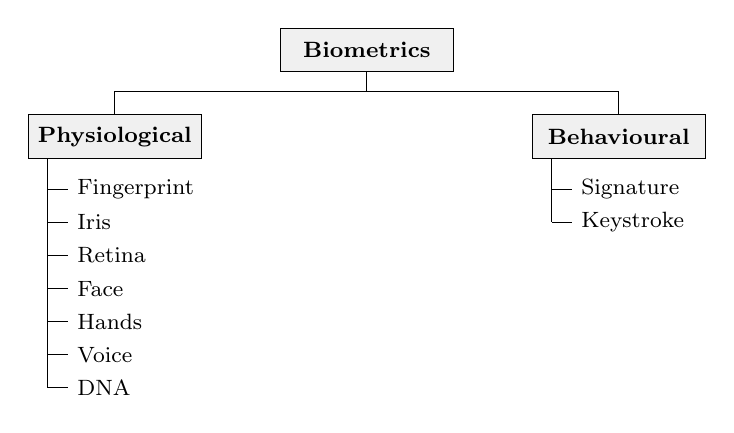
\begin{tikzpicture}[font=\footnotesize, level distance=0.95cm,
  bb/.style={draw, fill=gray!12, minimum width=2.2cm, minimum height=0.55cm, font=\footnotesize\bfseries}]
\node[bb] (root) at (3.2,0) {Biometrics};
\node[bb] (ph) at (0,-1.1) {Physiological};
\node[bb] (be) at (6.4,-1.1) {Behavioural};
\draw (root.south) -- ++(0,-0.25) -| (ph.north); \draw (root.south) -- ++(0,-0.25) -| (be.north);
\foreach \t [count=\i] in {Fingerprint, Iris, Retina, Face, Hands, Voice, DNA} {
  \node[anchor=west] (p\i) at (-0.6,-1.35-0.42*\i) {\t};
  \draw (-0.85,-1.35-0.42*\i) -- (p\i.west);
}
\draw (-0.85,-1.38) -- (-0.85,-1.35-0.42*7);
\foreach \t [count=\i] in {Signature, Keystroke} {
  \node[anchor=west] (b\i) at (5.8,-1.35-0.42*\i) {\t};
  \draw (5.55,-1.35-0.42*\i) -- (b\i.west);
}
\draw (5.55,-1.38) -- (5.55,-1.35-0.42*2);
\end{tikzpicture}
\end{center}
\begin{center}\small
\begin{tabularx}{\textwidth}{@{}l >{\raggedright}X >{\raggedright\arraybackslash}X@{}}
\toprule
Technique & What is measured & Remarks\\
\midrule
Fingerprint & ridges and valleys of the fingertip and their minutiae (ridge endings, bifurcations) & cheap and mature; cuts, dirt and worn skin cause rejections; prints can be lifted and copied\\
Iris & texture of the coloured ring around the pupil, from a camera & very distinctive, stable for life, contactless; costlier camera\\
Retina & pattern of blood vessels at the back of the eye & very accurate and hard to fake, but intrusive (eye close to the scanner)\\
Face & geometry of the face (distances between eyes, nose, mouth) & contactless, works from ordinary cameras; affected by lighting, expression, ageing, twins\\
Hands & hand geometry: lengths and widths of fingers and palm & simple and well accepted; not distinctive enough for 1:N identification\\
Voice & characteristics of the voice, from the shape of the vocal tract & usable over a telephone; affected by colds and noise, open to recordings\\
DNA & the DNA sequence of a cell sample & unique except for identical twins; needs a laboratory, not real time; forensics\\
\midrule
Signature & dynamics of signing: speed, pressure, stroke order, on a pad & familiar; varies over time and can be imitated with practice\\
Keystroke & typing rhythm: how long keys are held, time between keys & no extra hardware; can monitor a whole session; varies with fatigue and keyboard\\
\bottomrule
\end{tabularx}
\end{center}
The slides (Forouzan) list voice under physiological, because it depends on the vocal tract; Stallings puts voice pattern under dynamic (behavioural) biometrics, because it also depends on how a person speaks. In the exam, follow the slide tree and mention that voice has both aspects.

\textbf{Accuracy: FRR and FAR.} The accuracy of biometric techniques is measured with two parameters.
\begin{itemize}
  \item The \textbf{false rejection rate} (FRR) measures how often a person who should be recognised is not recognised by the system: $\mathrm{FRR} = \dfrac{\text{number of false rejections}}{\text{number of genuine attempts}} \times 100\%$.
  \item The \textbf{false acceptance rate} (FAR) measures how often a person who should not be recognised is recognised by the system: $\mathrm{FAR} = \dfrac{\text{number of false acceptances}}{\text{number of impostor attempts}} \times 100\%$.
\end{itemize}
A false rejection is an inconvenience (the genuine user tries again); a false acceptance is a security failure (an impostor gets in). The two rates are controlled by the same threshold and move in opposite directions. Raising the threshold demands a closer match, so fewer impostors pass (FAR falls) but more genuine users fail (FRR rises); lowering it does the reverse. The threshold at which the two rates are equal is the \textbf{equal error rate} (EER), a single number often used to compare systems: the lower the EER, the more accurate the technique. A bank vault is run at a high threshold (very low FAR, tolerating a higher FRR), a phone unlock or an attendance system at a lower one.
\begin{center}
\begin{tikzpicture}[font=\footnotesize, x=0.85cm, y=1cm]
\draw[->] (0,0) -- (8.6,0);
\node at (4.3,-0.4) {matching threshold: lenient $\longrightarrow$ strict};
\draw[->] (0,0) -- (0,3.3) node[above] {error rate};
\draw[very thick, warn, domain=0:8, samples=60] plot (\x, {3*exp(-0.6*\x)});
\draw[very thick, acc, domain=0:8, samples=60] plot (\x, {3*exp(-0.6*(8-\x))});
\node[warn, right] at (0.4,3.05) {FAR (impostors accepted)};
\node[acc, left] at (7.3,2.35) {FRR (genuine users rejected)};
\draw[dashed, gray] (4,0) -- (4,0.272);
\fill (4,0.272) circle (1.6pt) node[above=2pt] {EER};
\end{tikzpicture}
\end{center}

\begin{worked}[: computing FAR and FRR]
\textbf{Q.} A fingerprint system is tested with 1000 attempts by enrolled users, of which 30 are rejected, and 5000 attempts by impostors, of which 10 are accepted. (a) Find the FRR and the FAR. (b) The same matcher is used for identification against a database of 500 people, with the per-comparison FAR found in (a). What is the probability that an impostor matches at least one record?

\textbf{A.} (a) $\mathrm{FRR} = 30/1000 = \mathbf{3\%}$; \;$\mathrm{FAR} = 10/5000 = \mathbf{0.2\%}$.\\
(b) Each of the 500 comparisons is a false match with probability $0.002$, so
$\Pr[\text{at least one}] = 1 - (1 - 0.002)^{500} = 1 - 0.368 = \mathbf{0.632}$.\\
\emph{Check}: the expected number of false matches is $500 \times 0.002 = 1$, and $1 - e^{-1} = 0.632$. A FAR that is fine for 1:1 verification is useless for 1:N identification, which needs a far lower FAR.
\end{worked}

\textbf{Applications.} Biometrics is used for physical access control (the employee-only building of the slides; laboratories, data centres); logical access to phones and laptops; banking (cheque-signature verification as on the slides, biometric ATMs, Aadhaar-enabled payments); government identity (e-passports and border control, India's Aadhaar with fingerprints and iris); forensics (fingerprints, DNA); and attendance systems.

\textbf{Advantages.} The feature is always with the user and cannot be forgotten, lost or lent, so authentication is tied to the person rather than to an object or a secret; it is also convenient and fast.

\textbf{Disadvantages.} A biometric \textbf{cannot be changed if stolen}: a compromised password is replaced in a minute, but a person has ten fingers and two irises for life, so a leaked template is permanent damage. Features can be copied (prints lifted from a glass, photographs of a face, recordings of a voice), which requires liveness detection. Matching is approximate, so FAR and FRR are never both zero. Sensors cost money, some people cannot enrol (worn fingerprints, injuries), and a central database of templates raises \textbf{privacy} concerns: it can be used to track people across systems, some features reveal health information, and the database is a high-value target. For these reasons a biometric is best used as one factor of a multi-factor scheme, with the template kept locally (on the phone or the smart card) rather than in a central store.

\begin{fixbox}
\begin{itemize}
  \item Slide 13 (from Forouzan): ``If the original password is 6 digits and the salt is 4 digits \dots\ Eve now needs to make a list of 10 million items.'' A 10-digit value has $10^{10}$ (ten billion) possible values, not $10^{7}$; the precomputed list has $10^{10}$ entries. Also note that an attack on \emph{one} user, whose salt is read from the file, still needs only $10^6$ hashes.
  \item Slide 15: ``This kind of password makes eavesdropping and salting useless'' means that eavesdropping gains nothing and salting becomes \emph{unnecessary}, not that the one-time password defeats salting.
  \item Slide 23 says only that $s$ lies between 1 and $n - 1$; it must also be coprime to $n$, since otherwise $\gcd(v, n) > 1$ reveals a factor of $n$. Slide 24 lets $r$ be 0: Bob must reject $x = 0$, because the pair $x = 0$, $y = 0$ passes for both challenges.
  \item Slides 24--27 follow Forouzan's naming: $r$ is the ``commitment'' and $x$ the ``witness''. Most other texts call $x$ itself the commitment (or witness). Slide 27 also has ``passes the rest'' for ``passes the test''.
  \item Slide 28, second line of the proof: the last factor is printed $(s_2^2)^{c_2}(v_2^{c_k})$; it should be $(s_k^2)^{c_k}(v_k^{c_k})$.
  \item Slide 32: ``features that cannot be guessed, stolen, or shared'' is too strong. They cannot be forgotten or lent, but they can be copied (lifted fingerprints, photographs, recordings), and once copied they cannot be changed.
  \item Slide 34 divides both FRR and FAR by ``the total number of attempts''. FRR should be divided by the number of \emph{genuine} attempts and FAR by the number of \emph{impostor} attempts; dividing by the total mixes the two populations. Slide 33 also misspells ``Behavioural'' as ``Behaviorial''.
\end{itemize}
\end{fixbox}
